\documentclass[twocolumn,11pt]{article}
\usepackage[pdftex]{graphicx}  
\usepackage{amsmath}
\begin{document}
\title{Electronic structure of MgB$_2$}
\author{Mitsuaki Kawamura}
\maketitle


\section{Numerical condition}

The first-principles calculation based on density functional theory are performed
by using the Quantum ESPRESSO program package \cite{0953-8984-29-46-465901},
which employs plane waves and psudopotentials to describe the Kohn--Sham orbitals and the crystalline potential, respectively.
The plane-wave cutoff for a wave function is set to 35 Ry.
We employ the GGA-PBE functional \cite{PhysRevLett.78.1396}.
The ultrasoft pseudopotential \cite{PhysRevB.41.7892} \footnote{b\_pbe\_v1.4.uspp.F.UPF}
and the dataset of projector-augmented wave \cite{PhysRevB.50.17953} \footnote{Mg.pbe-n-kjpaw\_psl.0.3.0.UPF}
used in this study are obtained in Standard Solid State Pseudopotentials \cite{Prandini2018}.
They are originary included in the New Soft-Accurate NLCC pseudopotential library \cite{GARRITY2014446}
and Pslibrary 0.3.1 \cite{kucukbenli2014projector}. 
We set the ${\boldsymbol k}$-point grids of Brillouin-zone integrations with the optimized tetrahedron method \cite{PhysRevB.89.094515}
for the charge density and the partial density of states to 12$\times$12$\times$9 and 24$\times$24$\times$18, respectively.

\section{Result}

\begin{figure}[!tb]
  \begin{center}
    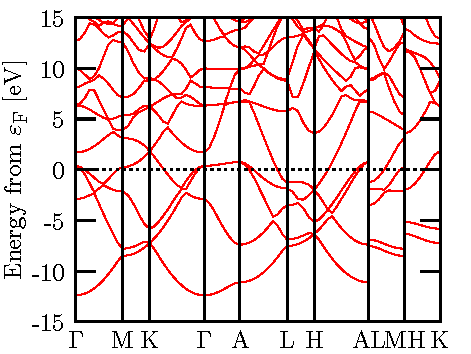
\includegraphics[width=8cm]{band.pdf}
    \caption{\label{fig_band}
      Band structure of MgB$_2$.
    }
  \end{center}
\end{figure}
%
Figure \ref{fig_band} shows the band structure of MgB$_2$.
%
\begin{figure}[!tb]
  \begin{center}
    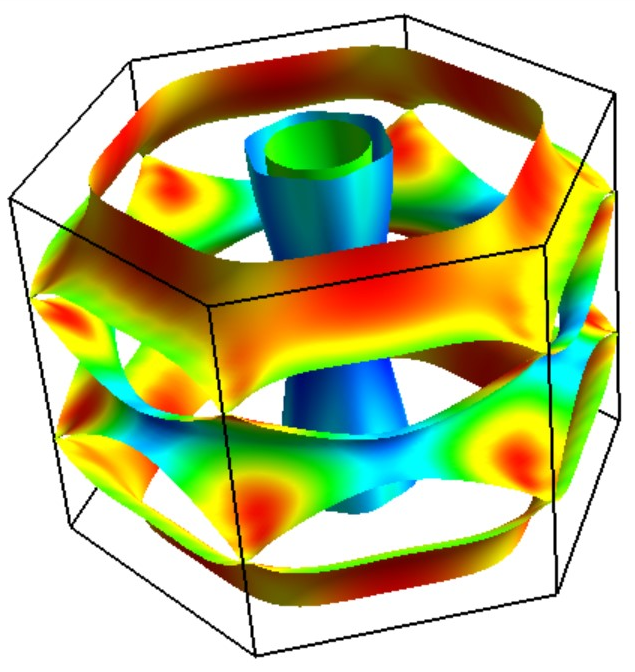
\includegraphics[width=5cm]{vfermi.png}
    \caption{\label{fig_fs}
      The fermi surface of MgB$_2$.
      Color scale indicates the absolute value of the Fermi velocity
      (red and blue mean the maximum and minimum of that velocity).
      We use FermiSurfer \cite{fermisurfer}
    }
  \end{center}
\end{figure}
%
This material has cylindirical Fermi surfaces at the center of the Brillouin zone and
three dimensional Fermi surfaces at the edge of the Brillouin zone (See Fig. \ref{fig_fs})
%
\begin{figure}[!tb]
  \begin{center}
    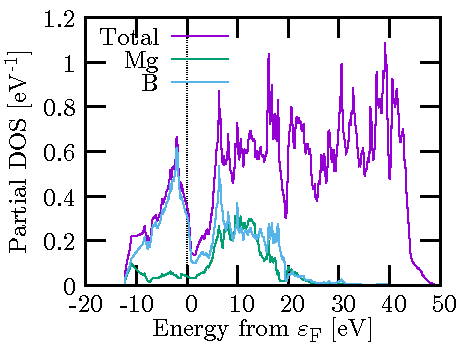
\includegraphics[width=8cm]{pdos.pdf}
    \caption{\label{fig_pdos}
      Partial density of states of MgB$_2$.
      Mgenta, green, blue lines indicate
      the total, Mg-, and B-projected density of states, respectively.
    }
  \end{center}
\end{figure}
%
Partial density of states is shown in Fig. \ref{fig_pdos}
%
\begin{figure}[!tb]
  \begin{center}
    \includegraphics[width=2.7cm]{{tmp.pp_K001_B002}.png}\includegraphics[width=2.7cm]{{tmp.pp_K001_B003}.png}\includegraphics[width=2.7cm]{{tmp.pp_K001_B004}.png}
    \caption{\label{fig_orb}
      The Kohn--Sham orbitals of (left) second, (center) third,
      and (right) forth band at $\Gamma$ points, respectively.
      We use VESTA \cite{Momma:db5098} for displaying this figure.
    }
  \end{center}
\end{figure}
%
Figure \ref{fig_orb} shows the Kohn--Sham orbitals at $\Gamma$ point.

\bibliographystyle{unsrt}
\bibliography{report}
\end{document}
